\chapter{Анализ данных эксперимента}\label{chapt3}

После проведения экспериментальных исследований влияния радиуса закругления рабочей кромки и шага резания на составляющие силы, возникающей на дисковом инструменте, при механическом разрушении льда, получен набор <<сырых>> данных, который включает в себя:
\begin{itemize}
	\item фотографии осколков;
	\item графики переходных процессов для каждого сочетания факторов.
\end{itemize}

Дальнейшее их использование предполагает обработку и оценку корректности методами математики и статистики, такими как:
\begin{itemize}
	\item фильтрация постоянной составляющей;
	\item отброс грубых ошибок;
%	\item оценка дисперсии;
	\item усреднение значений;	
	\item сглаживание.
\end{itemize}

Далее в это главе процесс обработки и оценки адекватности данных будет приведен последователь.

\section{Фильтрация и сглаживание переходных процессов резания льда}\label{sect3_1}

Чтобы исключить <<дрейф нуля>>\footnote{смещение сигнала относительно нуля из-за присутствия постоянной составляющей.} необходимо убрать из сигнала переходного процесса постоянную составляющую. Самый простой способ это сделать, перевести сигнал в частотную область, например быстрым преобразованием Фурье (БПФ) \cite{BPF,BPFEng}. Воспользуемся следующей формулой для его реализации:
\begin{equation}\label{eq:FFT}
X(k)=\sum_{j=1}^{N} x(j)\cdot\omega_{N}^{(j-1)\cdot(k-1)}
\end{equation}
где $ N $ "--- количество точек в снятом переходном процессе; $ \omega_{N} = e^{\frac{-2\pi i}{N}} $ "--- корень $ N $-ой степени; $ X(k) $ "--- ряд фурье, образ входного сигнала; $ x(j) $ "--- входной сигнал (записанный переходный процесс).

В пакете прикладных программ matlab вычисление БПФ сводится к нескольким строчкам кода. Приведем пример вычисления со сдвигом нулевой частоты в середину спектра:
\begin{lstlisting}
	X = fft(x);
	X = fftshift(X);
\end{lstlisting}

Исходя из свойств преобразования Фурье, таких как линейность и симметричность, для более наглядного представления спектра сигнала можно без последствий отбросить отрицательную часть, тоесть ровно половину массива \verb|X|. 
\begin{lstlisting}
	X = X(end/2+1:end);
\end{lstlisting}

После перехода в частотную область, сигнал представляет собой набор значение частот всех гармоник образующих исходный сигнал. Можно графически оценить спектр переходного процесса, например для вертикальной составляющей силы, при радиусе закругления $ R=0,5 $ и шаге резания $ t=10 $, рисунок \ref{img:Spectrum}. Как известно из главы \ref{chapt2}, частота дискретизации АЦП равна 100~Гц. На графике же мы видем максимальную частоту 50~Гц, это обусловленно симметричностью преобразования Фурье. 
\begin{figure}[ht] 
	\center
	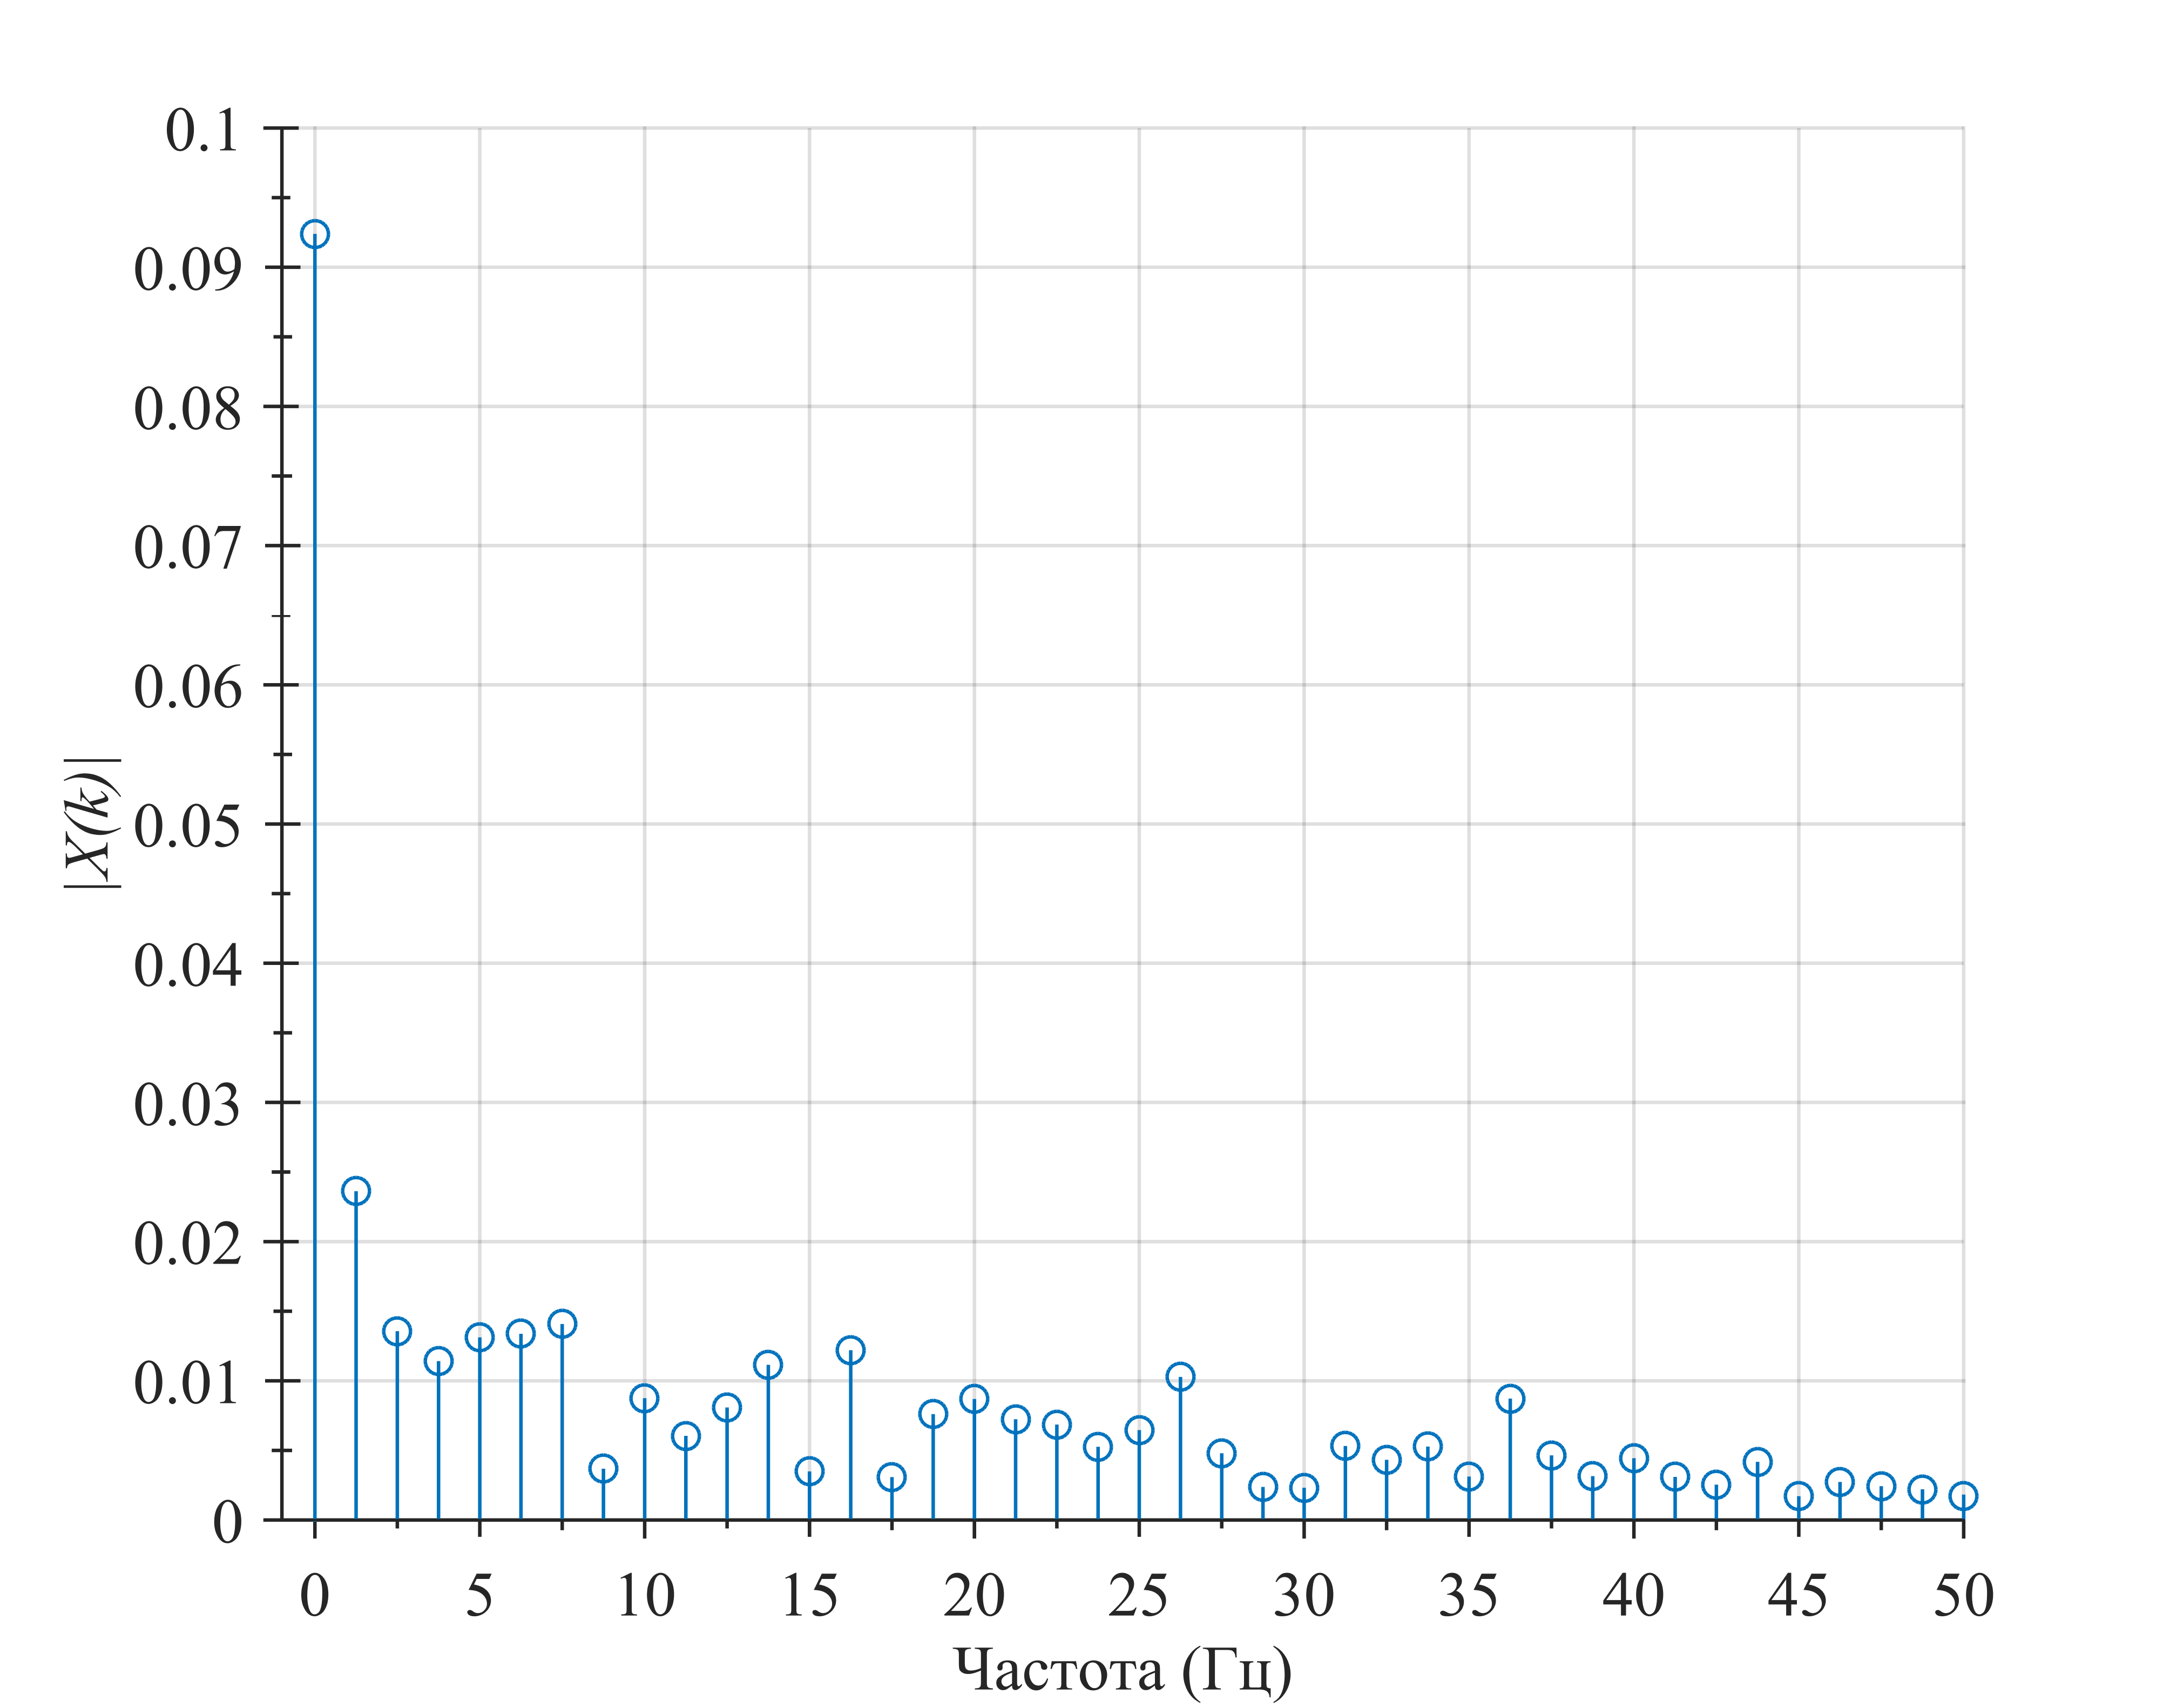
\includegraphics{Spectrum}
	\caption{Спектр сигнала переходного процесса разрушения льда, для вертикальной составляющей силы. При $ R=0,5 $ и $ t=10 $} 
	\label{img:Spectrum}  
\end{figure}

Как видно из рисунка \ref{img:Spectrum} при нулевой частоте заметен значительный всплеск амплитуды. Что обуславливает присутствие в сигнале некой постоянной составляющей с амплитудой равной 0,0926.  Для ее удаления из сигнала достаточно просто обнулить первый элемент в полученном ряду Фурье (значение амплитуда для составляющей с частотой 0, тоесть постоянной) \verb|X(1)=0;| и выполнить обратное преобразование с помощью формулы:
\begin{equation}\label{eq:iFFT}
x(j)=\frac{1}{N}\sum_{k=1}^{N} X(k)\cdot\omega_{N}
\end{equation}

Средствами matlab это же действие выполняется путем обратного сдвига и обратного же БПФ:
\begin{lstlisting}
X = ifftshift(X);
x = ifft(X);
\end{lstlisting}
\begin{figure}[ht] 
	\center
	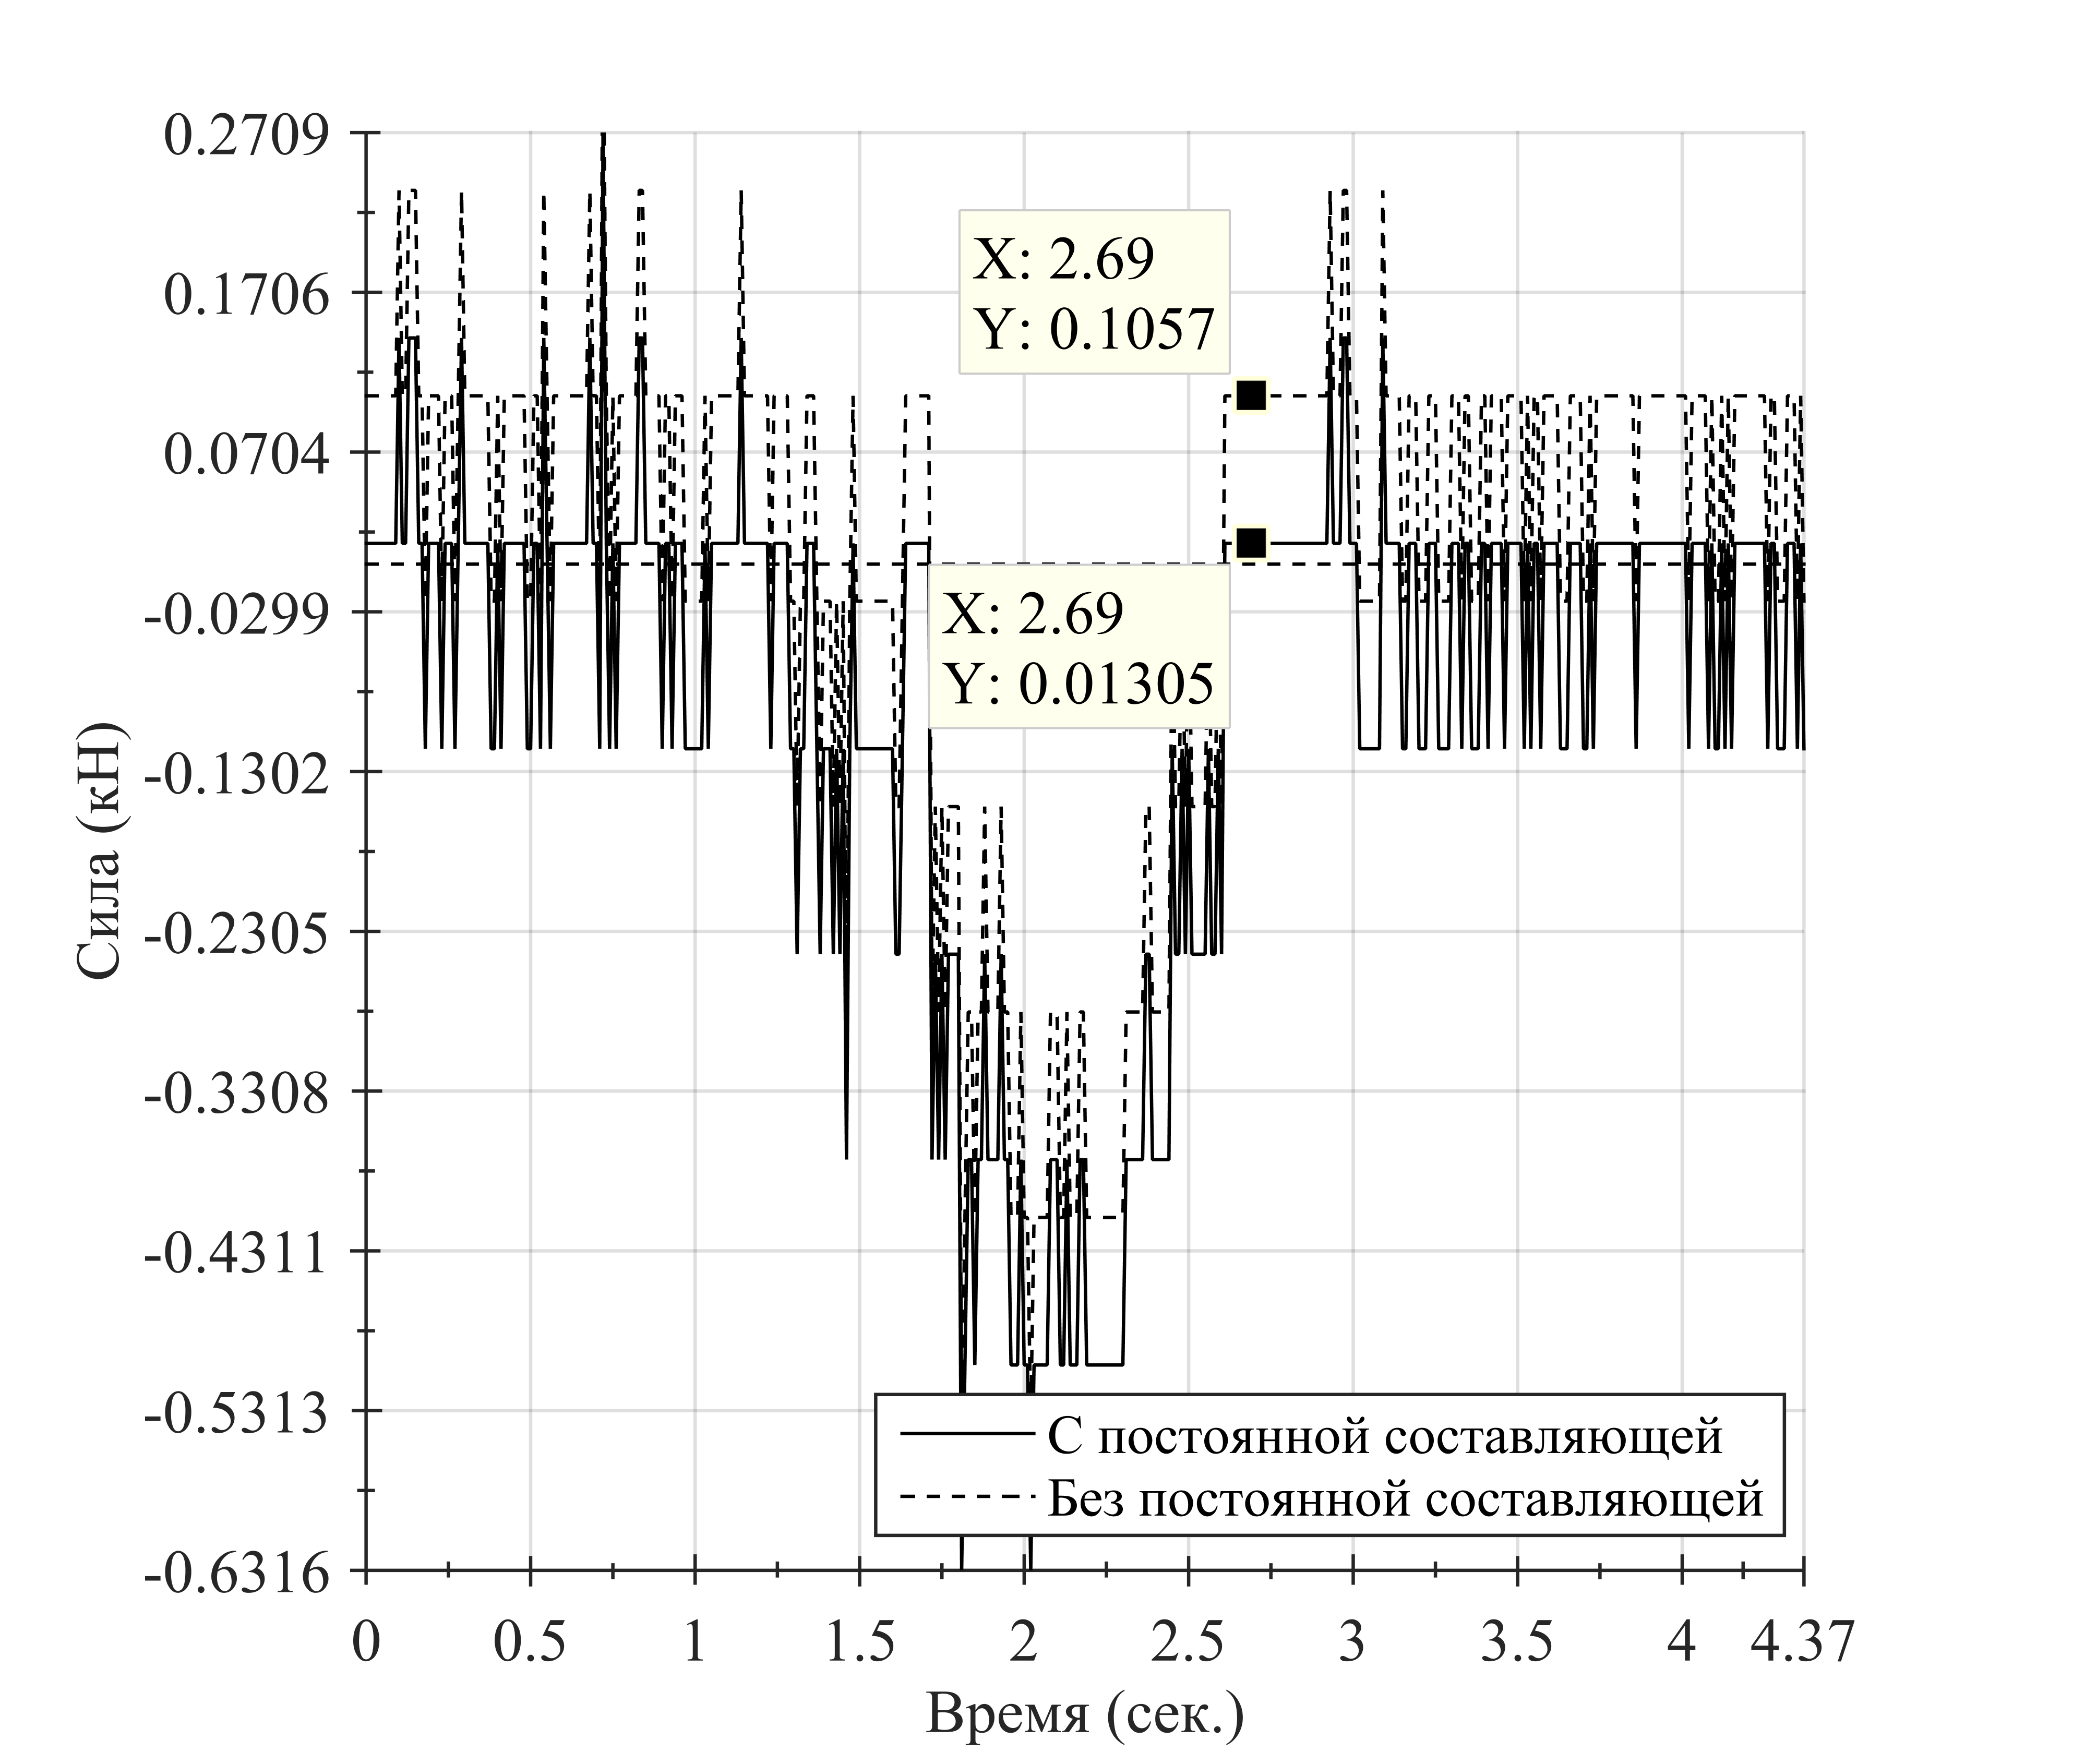
\includegraphics{SignalRaw}
	\caption{Переходный процесса разрушения льда} 
	\label{img:SignalRaw}  
\end{figure}

Результат работы данного алгоритма приведен на рисунке \ref{img:SignalRaw}. Как видно из графика, не обработанный сигнал (сплошная линия) имеет смещение относительно обработанного (штриховая линия) ровно на 0,0926 что соответствует амплитуде постоянной составляющей, найденной выше. Все остальные записанные сигналы обработаем подобным образом.

\section{Отброс грубых ошибок}\label{sect3_2}

Для улучшения точности оценки переходного процесса и снижения влияния всевозможных внешних факторов целесообразно применить к полученному набору точек (сигналу) алгоритм отброса грубых ошибок \cite{LvovStat}. Суть алгоритма заключается в использовании метода максимального относительного отклонения:
\begin{equation}\label{eq:MOO}
	\tau=\frac{|x_i-\bar{x}|}{\bar{\sigma_x}},
\end{equation} 
где $ x_i $ "--- крайний (наибольший или наименьший) элемент сигнала; $ \bar{x} $ "--- среднее значение сигнала; $ \sigma_x $ "--- СКО сигнал (расчитывается по формуле \ref{eq:sigma_x}).

Сравнивая $ \tau $ с критическим значением $ \tau_{(p,n)} $, рассчитанным по формуле \ref{eq:tau_krit}, можно сделать вывод является ли наблюдение грубой погрешностью или нет.
\begin{equation}\label{eq:tau_krit}
	\tau_{(p,\ n)}=\frac{t_{(p,\ n-2)}\cdot\sqrt{n-1}}{\sqrt{n-2+|t_{(p,\ n-2)}|^2}}
\end{equation}
где $ t_{(p,\ n-2)} $ "--- критическое значение распределения Стьюдента при доверительной вероятность $ q=1-p $; $ n $ "--- количество наблюдений в сигнале переходного процесса.

Критическое значение распределения Стьюдента в ППП matlab можно вычислить с помощью функции \lstinline{tinv()}. 
\begin{lstlisting}
	t = tinv(p / 100, n - 2);
\end{lstlisting}
где \lstinline{p} "--- вероятность; \lstinline{n} "--- количество наблюдений.

Имеет смысл ввести три группы наблюдений, удовлетворяющих следующим условиям:
\begin{enumerate}
	\item $ \tau \leqslant \tau_{(5\%,\ n)} $ нельзя отсеивать.
	\item $ \tau_{(5\%,\ n)} < \tau < \tau_{(0,1\%,\ n)} $ можно отсеять, если в пользу этой процедуры имеются и другие соображения.
	\item $ \tau > \tau_{(0,1\%,\ n)} $ отсеиваются всегда.
\end{enumerate}

Таким образом имеем алгоритм отброса грубых ошибок выглядящий следующим образом:
\begin{enumerate}
	\item Из наблюдаемых значений выбирается максимальное и минимальное значение сигнала.\label{enum:alg_DGE_1}
	\item Максимум и минимум сравниваются по модулю и выбирается наибольшее.
	\item Рассчитывается $ \tau $ по формуле \ref{eq:MOO}.
	\item Вычисляются критические точки $ \tau_{(0,1\%,\ n)} $ и $ \tau_{(5\%,\ n)} $ по формуле \ref{eq:tau_krit}.
	\item Проверяется условие $ \tau > \tau_{(0,1\%,\ n)} $ если выполняется исключаем наблюдение из массива точек и переходим к пункту \ref{enum:alg_DGE_1}.
	\item Проверяем условие $ \tau_{(5\%,\ n)} < \tau < \tau_{(0,1\%,\ n)} $ если выполняется смотрим другие факторы и принимаем решение, если не отбрасываем переходим к пункту \ref{enum:alg_DGE_1}.
	\item Оставшиеся точки и есть сигнал с отброшенными грубыми ошибками.
\end{enumerate}

Алгоритм реализованный средствами пакета прикладных программ matlab представлен в приложении \ref{Appendix:FPE:DGE}, листинг \ref{list:DropGrossError}.





% Алгоритм встроенными средствами
%\begin{figure} [htbp]
%	\center
%	\begin{tikzpicture}
%		[line/.style ={draw,-latex, line width=1pt},]
%		\node [start_stop] (start) {Начало};
%		\node [block,below = of start] (max) {$	\cfrac{\max | x - \bar{x} |}{\bar{S}} $};
%		\node [block,below = of max] (t) {$ t_{(5\%,\ n-2)} $\\$ t_{(0,1\%,\ n-2)} $};
%		\node [start_stop,below =of t] (stop) {Конец};
%		
%		\begin{scope}[every path/.style=line]
%			\path (start) -- (max);
%			\path (max) -- (t);
%			\path (t) -- (stop);
%			%\path (decide) -- node [midway] {no} (stop);
%		\end{scope}
%	\end{tikzpicture}
%	\caption{Блоксхема} 
%\label{img:Block}  
%\end{figure}




\section{Усреднение повторных опытов}\label{sect3_3}


В задачах контроля и управления технологическими процессами, учета электроэнергии, контроля за работоспособностью и функционированием силовой коммутационной техники и прочих важно знать энергетические свойства переменного сигнала, характеризующие  его способность совершать работу. Таким параметром переменного сигнала является  его среднеквадратичное значение. Не менее широко применяются также термины «действующее значение», «эффективное значение». В дальнейшем мы будем использовать термин «действующее значение».
\begin{equation}\label{eq:rms}
F_\text{Д}=\sqrt{\frac{1}{n}\cdot\sum_{i=1}^{n} F_i}
\end{equation}


Из параграфа \ref{sect2_2} известно, что для каждый опыт повторялся 5 раз, для учета неизвестных факторов, а это значит что данные необходимо усреднить.

Точечную оценку величины действующей силы можно вычислить через:
\begin{equation}\label{eq:x_ocenka}
\hat{F}=\frac{1}{n}\sum_{i=1}^{n} F_i,
\end{equation}
где $ n $ "--- число повторных опытов, $ F_i $ "--- измеренное значение в отдельном опыте \cite{Zajigaev}.

Среднеквадратичное отклонение точечной оценки 
Оценить точность позволит относительная погрешность измерений, вычисляемая по следующее формуле:
\begin{equation}\label{eq:Error}
\varepsilon=\frac{1}{n}\sum_{i=1}^{n} \frac{\left| x_i-\bar{x}\right| }{\bar{x}}\cdot100\%
\end{equation}